
\chapter*{Machine Learning with Neural Networks}
\addcontentsline{toc}{chapter}{Machine Learning with Neural Networks}

\section*{Machine Learning Terminology}
\addcontentsline{toc}{section}{Machine Learning Terminology}
In this lab, we\rq ll dip our toes in the field of machine learning. In very loose terms, machine learning boils down to the process of using general algorithms to model (sometimes complicated) relationships between system parameters. In a typical scenario we\rq ll have an observable quantity which is thought to relate to a set of input data. For example, suppose you have a bunch of pictures of pets that you want to classify by the type of animal in the picture (cat, dog, parrot, etc.). The observable quantity is the type of animal, and the data consists of the pixel locations and values in the picture.\\

To get started on this picture classification project, you could manually classify a bunch of pictures by the type of animal in them and then provide that training data to the machine learning algorithm. The algorithm uses the training data to come up with a model that takes a picture as input, and predicts the type of animal in the pictures. You can then use the output model to automatically classify the rest of your pet pictures. This process is called supervised learning.

Supervised Learning: The researcher provide a machine learning algorithm with a \rq\rq training\lq\lq data set where the outcomes for each of the given data inputs are known, and the algorithm comes up with a function relating the inputs and outputs that can then be used on new data

Model: The output of a machine learning algorithm that represents a relationship between inputs and outputs.

The picture-sorting procedure outlined above is an example of a classification problem. Classification algorithms are designed to fit sets of data into discrete bins (cat, dog, etc.). In contrast, regression algorithms aim to predict a value based on the input data. For example, you might try to use machine learning to predict the temperature tomorrow. In this case, the measurable quantity is a number representing the temperature, and the input data would be things like the historic temperature record, the date, the location, recent weather, etc.

Classification: The measurable quantity is restricted to a discrete set of values.
Regression: The measurable quantity is allowed to take on a continuous range of values.

Sometimes, you don\rq t have a measurable quantity you want to predict from your data set, but rather want to explore the structure of the data itself. For example, say Facebook wants to divide their users into groups of people with similar demographics so they can target advertising to these groups. They want to be able to say something like "this ad is likely to be interesting to demographic group $\alpha$ but uninteresting to group $\beta$." But they don\rq t know the best way to define the groups $\alpha$ and $\beta$. This is a job for a clustering algorithm, which is a type of unsupervised learning. Facebook could feed a bunch of information about a set of people into a clustering algorithm, and the algorithm would return suggestions for how to assign those people to groups \rq\rq similar \lq\lq demographics (i.e. tell you how to define groups $\alpha$ and $\beta$ above). Once they\rq ve classified the data into groups, they could then use a supervised machine learning algorithm to predict which groups might be likely to click on which advertisements.

Unsupervised Learning: An algorithm that looks for patterns or groupings in a set of data without respect to any presuppositions about the data.

Clustering: A type of unsupervised learning algorithm that separates similar data into groups or categories.


\begin{problem}\label{P13.1} Explain the machine learning concepts introduced above to a TA.\end{problem}
There are many, many more ideas in machine learning. You can take many full courses on the subject. But just to get the flavor of how this works, let\rq s tackle some specific problems using a common machine learning technique referred to as a neural network.


\section*{Linear Regression}
\addcontentsline{toc}{section}{Linear Regression}

A computational neural network can be thought of as an extension of linear regression. Linear regression finds a linear function which maps an input, $x$, onto an output, $y$. Circles are often used to represent the nodes (values) of a neural network. Using that notation, a linear regression mapping would be represented this way:

Questions that linear regression can answer are along the lines of this: given a set of known inputs with corresponding known outputs, can one predict what the output will be for a new input that wasn't part of the original set? As an example, perhaps you are trying to correlate exam scores with the amount of time students studied for the exam as shown in Table 13.1.
% tu fote dac z strony 96
You could make a plot of the data and fit a line to it as shown in Fig. 13.1. Then you could use your fit to make a prediction for a student not in the given data set, such as \rq\rq Given a time $x=2.7$ hours, the expected exam score would be $y=53$ percent.\lq\lq The linear fit is typically done by choosing the slope and intercept parameters to minimize some cost or loss function, for example the squared error.\\

Simple linear prediction is often insufficient. For example, this linear fit will predict a negative score for particularly low values of study time, which is nonsensical. So it would make sense to apply a nonlinear function after the linear fit, something like $y=\max (0, z)$ where we are now using the symbol $z$ to represent the value that is given from the linear fit, $z=w x+b$, so we can continue to use the symbol $y$ for the final output. (We are using the letter $w$ to represent the slope of the line for reasons made clear below.) Applying that particular nonlinear function is equivalent to saying, "Set $y$ to 0 if $z$ is negative, otherwise use $y=z$ ".
In a neural network, a function applied after the linear fit is called an activation function, and that particular activation function is probably the most commonly used one. It is called the relu function, which stands for rectified linear unit. Other activation functions are also frequently used. For example, another common situation is when the output value must be between 0 and 1 ; in that case a nonlinear function called a sigmoid function, is used to map all the $z$ values (potentially ranging from $-\infty$ to $+\infty$ ) to real values of $y$ between 0 and 1 .
\marginpar{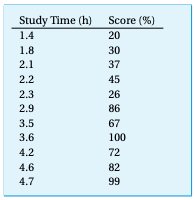
\includegraphics[width=\marginparwidth]{tab1301}\captionof{table}{Table of exam scores vs. study time.}\label{fig:52}}
\marginpar{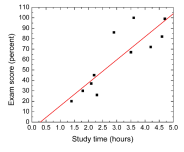
\includegraphics[width=\marginparwidth]{fig1301}\captionof{figure}{Simple linear fit of the test data shown in Table 13.1.}\label{fig:53}}
\section*{Multiple input linear regression}
\addcontentsline{toc}{section}{Multiple input linear regression}
Linear regression can also be done with multiple inputs. Continuing the exam score example, additional inputs could represent other known quantities such as how much sleep the student got the night before the exam, the student's class attendance, the student's grades on homework and past exams, etc. The situation might now look like this; we are using $z, y$ notation at the final node to indicate that the output node has both pre- and post-activation values.
%obrazek stron 97
The linear function which would now be fit is $z=w_{1} x_{1}+w_{2} x_{2}+w_{3} x_{3}+w_{4} x_{4}+b$, and then an activation function could be applied to the value of $z$ to obtain $y$. The slopes of the linear regression are now called weights, hence the symbol $w$. Each $w$ is represented in the figure by an arrow. The optimal values of the parameters $w_{1}, w_{2}, w_{3}, w_{4}$, and $b$ will be calculated together using known data to minimize a cost function.
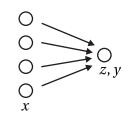
\includegraphics[width=4cm]{page97}
\section*{Neural networks}
\addcontentsline{toc}{section}{Neural networks}
A neural network is this same idea as multiple regression, just expanded to multiple layers. The layers between input and output are called hidden layers. Each hidden layer could have its own activation function. Post-activation values of the nodes of the hidden layers are called the activations of the nodes and are represented by the letter $a$. Here's an example of a three layer neural network; by convention, the input layer of $x$ 's is not counted in the number of layers of the network.
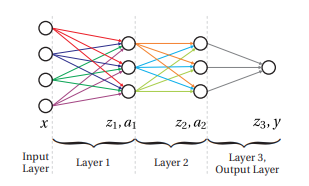
\includegraphics{fig1302}\captionof{figure}{Example of a fully connected three-layer network.}
Note that in this example, layer 1 is a collection of 15 parameters (4 $w$ \rq s and 1 $b$ for each of the three nodes in layer 1 ), an activation function, and 3 nodes. This nomenclature is not necessarily uniform; some people may just refer to the nodes themselves when discussing a layer. Also, sometimes the $a$ and $z$ values are counted as separate layers, in which case this example would be called a six-layer neural network. The structure of the network, meaning the number of layers, and the number of nodes in each layer, and their activation functions, is chosen with the goal of obtaining the best possible predictions. It is fairly common, however, to reduce the number of nodes in each layer as one moves from input to output as in this example here.

\section*{More complicated layers}
\addcontentsline{toc}{section}{More complicated layers}
The layers shown in Fig. $13.2$ are termed fully connected layers, meaning each node of the previous layer is connected via an arrow (i.e. a $w$ ) to each node of the next layer. Incidentally, this type of network is called a multilayer perceptron. More complicated layers can also be used. One type of layer which is frequently used in image analysis is called a convolutional layer. A color image input is represented numerically by a 3 -dimensional array: 2 dimensions for horizontal and vertical values, plus a third dimension specifying whether the given numbers refer to the $\mathrm{R}, \mathrm{G}$, or $\mathrm{B}$ color channel. A convolutional layer takes a 3-dimensional array as an input, does an operation on it, and then passes a new 3 -d array to the next layer. One can have multiple convolutional layers in a network, but to convert from a convolutional layer to a fully connected layer at some point, the data must be "flattened" from a $3-d$ array to a $1-d$ set of values.
\marginpar{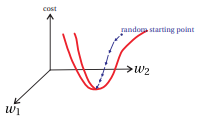
\includegraphics[width=\marginparwidth]{fig1303}\captionof{figure}{Taking steps by adjusting the $w_{1}$ and $w_{2}$ parameters along the negative gradient direction to find the minimum of the cost function.}\label{fig:54}}

\section*{Gradient descent}
\addcontentsline{toc}{section}{Gradient descent}
In the specific neural net shown in Fig. 13.2, layer 1 contained 15 fitting parameters. Similarly, layer 2 contains 12 parameters and layer 3 has 4 parameters. (Take a moment to look at the figure and make sure these numbers make sense to you.) Therefore 31 total parameters need to be optimized using the input data. For more complicated neural nets, it is not uncommon for there to be hundreds of thousands of fitting parameters! How are these to be optimized? The process is typically done using the gradient descent method (or a close relative of it).
Gradient descent is an iterative process whereby the location of the minimum of a function (e.g. the cost function) is found by taking steps along the "downhill" direction, i.e. the direction of the negative gradient. This is most easily visualized with a function of two parameters, say $w_{1}$ and $w_{2}$, as illustrated in Fig 13.3.
At each step in the iteration, the cost function is computed based on the current values of $w_{1}$ and $w_{2}$, the gradients of the cost function with respect to $w_{1}$ and $w_{2}$ are computed at the present location of $w_{1}$ and $w_{2}$, and then the values of $w_{1}$ and $w_{2}$ are updated according to:
\begin{equation*}
\begin{aligned}
&w_{1, \text { next }}=w_{1}-\alpha \frac{d(\cos t)}{d w_{1}} \\
&w_{2, \text { next }}=w_{2}-\alpha \frac{d(\cos t)}{d w_{2}}
\end{aligned}
\end{equation*}
For known activation functions and a known cost function, the gradients can be automatically computed by the machine learning software in an interesting backpropagation process that minimizes calculation time, but is beyond the scope of this lab.


\section*{Hyperparameter tuning and training/validation sets}
\addcontentsline{toc}{section}{Hyperparameter tuning and training/validation sets}
In those equations, the symbol $\alpha$ is called the learning rate and must be carefully chosen. It describes how large a step is taken during each iteration. Too small of a value and the process will take many iterations to converge. Too large a value and the steps may overshoot the minimum that is being sought. The input $\alpha$ is an example of a hyperparameter, meaning a parameter that affects the machine learning but is not automatically optimized by the algorithm itself (unlike the $w_{\text {'s }}$ and $b$ 's). Other examples of hyperparameters include the number of layers, number of nodes in each layer, the activation functions, and even the cost function itself. Sometimes these hyperparameters can be tuned in a systematic way, but often selecting the best hyperparameters involves a degree of trial and error.
How can one decide which hyperparameters are best? It would be tempting to just look at the cost function and pick the hyperparameters which produce the lowest possible value. However, with potentially hundreds of thousands of fitting parameters, the danger of overfitting the data is very real, meaning you could end up with a set of parameters that do a fantastic job on fitting the given data, but which make horrible predictions on any new data. To guard against that, the known data is typically separated into a training set and a validation set. The validation set is also known as the development set or "dev set"; sometimes it is also called the "test set," although at times "test set" refers to a third set used  for additional testing after the model is complete so we will avoid that usage. The training set is used to optimize the network parameters to minimize the cost function, i.e., to "train the model", and then the trained neural network is checked against the validation set to make sure the network can be relied on to give predictions which make sense.

\section*{The Keras library}
\addcontentsline{toc}{section}{The Keras library}

Fortunately, the many steps involved with training and testing neural networks are greatly simplified using machine learning libraries, of which one of the most used for Python is called keras. The examples below all use keras. Use this pip install command:
\begin{lstlisting}
pip install keras
\end{lstlisting}
Use these additional commands if needed:
\begin{lstlisting}
pip install tensorflow
pip install -U numpy
\end{lstlisting}
If keras still does not work after those commands, you may have a version conflict. In that case, see Appendix A for some basics about environments in Anaconda and download an environment file from our website, which should help. Install and activate it, and then the specified libraries should work together.

\section*{Example 1: Predicting exam scores}
\addcontentsline{toc}{section}{Example 1: Predicting exam scores}
Here is what the code would look like to use a neural net framework to analyze the exam score vs. study time data set given above, and then to make a prediction for $x=2.7$ hours. As a quick note about notation, while the letters $x$ and $y$ are commonly used to refer to a single input data point and its corresponding output, the collections of all inputs and outputs are usually referred to as capital $X$ and $Y$.
This code sets up a 1 layer neural network with 1 node in the layer, which receives a single input from an input layer. The model=Sequent ial () command creates a sequential (normal) neural net with name model. The layer is created via the model.add (Dense $(1, act ivation='linear', input_dim=1)$) command, where the first 1 refers to the number of nodes in the layer and the second 1 designates the size of the input layer (a single input node). We use sgd as the optimizing routine, which stands for stochastic gradient descent, and a mean squared error cost (or loss) function. For this simple example we are not bothering with a validation set and we have used a linear activation function (meaning the identity, $y=z$ ) instead of a relu one. The predicted $y$ for $x=2.7$ should be about $y \approx 54.4$.
\begin{lstlisting}
import numpy as np
from keras.models import Sequential
from keras.layers import Dense
from keras import optimizers

data = np.array([[1.4, 20.], [1.8, 30.], [2.1, 37.], [2.2, 45.],
				[2.3,26.], [2.9, 86.], [3.5, 67.], [3.6, 100.],
				[4.2, 72.], [4.6, 82.], [4.7, 99.]])
				
[X_train,Y_train] = data.transpose()

model = Sequential()
model.add(Dense(1, activation='linear', input_dim=1))
sgd = optimizers.sgd(lr=0.03) #lr is the learning rate
model.compile(loss='mean_squared_error',optimizer=sgd)

#this command does the minimization
model.fit(X_train, Y_train, epochs=100, verbose=1)

#displays some info, note there are only 2 fitting parameters
model.summary()

# the predict function on the next line assumes an
# array of inputs so we need to put 2.7 inside an array
x = np.array([2.7])

#... and predicted_y is likewise an array of predicted outputs
predicted_y = model.predict(x)

print('For x={:f} the predicted y is: {:f}'.format(float(x),float(predicted_y)))
\end{lstlisting}


\begin{problem}\label{P13.2}Execute the code above, and examine the output. Explain to the TA what
the code does.\end{problem}



\section*{Example 2: Predicting median home prices}
\addcontentsline{toc}{section}{Example 2: Predicting median home prices}
A commonly used data set for testing machine learning algorithms, and one built into keras, is that of Boston home prices from the $1970 \mathrm{~s}$. It involves 13 metrics taken for 506 different communities in the Boston area, along with the median home price for the community. Reading it into your code from the keras . dat asets as is done below will automatically sort the data into 404 training data points and 102 validation data points with the 13 metrics as the $X$ vector and the median home price as $Y$. Technically $X$ is a 2-d array, because each $x$ is a collection of 13 pieces of information, and $X$ is the collection of all $x$ 's for all 404 training data points.\\
This code sets up a five-layer neural network with $30,15,8,5$, and 1 nodes per layer respectively. There are 1,064 total fittable parameters. Notice how each layer is just added via a model. add command, and only the first input layer needs to have input$\_$dim specified ( which is the number of nodes in the input layer ). In this example a dam is used as the optimizing routine; it is a slightly more sophisticated version of gradient descent and is a popular choice for many
applications.

\begin{lstlisting}
import numpy as np
from keras.models import Sequential
from keras.layers import Dense
from keras import optimizers
from keras.datasets import boston_housing

(X_train, Y_train), (X_validate, Y_validate) = boston_housing.load_data()

#description here: https://github.com/eric-bunch/boston_housing

print(X_train.shape)
print(Y_train.shape)
print(X_validate.shape)
print(Y_validate.shape)

model = Sequential()
model.add(Dense(30, activation='relu',input_dim=13))
model.add(Dense(15, activation='relu'))
model.add(Dense(8, activation='relu'))
model.add(Dense(5, activation='relu'))
model.add(Dense(1, activation='linear'))
optimizer_choice = optimizers.adam(lr=0.05)
model.compile(loss='mean_squared_logarithmic_error',
optimizer=optimizer_choice, metrics=['mse'])
model.fit(X_train, Y_train, batch_size=32, epochs=50, verbose=1)
model.summary()
score = model.evaluate(X_validate, Y_validate, verbose=0)

print('The loss value and accuracy of the test set is: ' + str(score))

#prediction for a specific input
test_num = 27 #randomly chosen number
x = np.array([X_validate[test_num]])
predicted_y = model.predict(x)
print('For input parameters x = ')
print(X_validate[test_num])
print('the predicted y (median value of home, in $1000s) is:
	{:f} '.format(float(predicted_y)))
print('and the actual y value was: {:f}'
	.format(float(Y_validate[test_num])))
\end{lstlisting}

\begin{problem}\label{P13.3} Execute the code above, and examine the output. Explain to the TA what
the code does.\end{problem}


\section*{Example 3: Predicting handwritten digits}
\addcontentsline{toc}{section}{Example 3: Predicting handwritten digits}
Now we will do a more complicated example using image classification with the
MNIST data set which contains images of handwritten digits, each labeled with
the answer for the correct digit. Our neural net will use the data set to learn how
to recognize the digits. Each data point is a 28×28 pixel monochrome image.
Reading the data set into your code from the keras.datasets as is done below will
automatically sort the data into 60,000 training data points and 10,000 validation
data points with the with the pixel values as $X$ and the correct digit as $Y$ .\\

This code sets up a 4 layer neural network where the first two layers are
of the convolutional type mentioned above (convolutional hyperparameters:
32 convolutional \rq\rq filters\lq\lq and a 3 × 3 convolutional grid for each layer), followed by two regular (dense) layers of sizes 128 and 10, respectively. The output layer has size 10 because for categorizing data like this, the output of the
neural net needs to be 10 different outputs, each one corresponding to the likelihood of the image being a particular digit. So instead of 3, 5, or 6, our outputs
need to be things like $[0 0 0 1 0 0 0 0 0 0]$, $[0 0 0 0 0 1 0 0 0 0]$, and
$[0 0 0 0 0 0 1 0 0 0]$.
The input shape of the $X$ values must be specified for the first layer; after that, keras is smart enough to determine the needed array sizes and shapes. The output of the second layer must be flattened prior to going into the third layer. Some of the layers employ dropout which helps prevent overfitting. Pooling is a technique to reduce the size of the convolutional arrays. The output layer, as mentioned above, needs to have 10 separate outputs. The softmax activation choice for the final layer makes it so the 10 output values sum to 1 and can be interpreted as probabilities. The cost function is categorical$\_$crossentropy which is the typical choice for sorting data into categories. Because this is a more complicated example, some additional comments are given in the code.

\begin{lstlisting}
import numpy as np
from matplotlib import pyplot as plt
from keras.models import Sequential
from keras.layers import Dense, Dropout, Flatten
from keras.layers import Conv2D, MaxPooling2D
from keras.utils import np_utils
from keras.datasets import mnist

(X_train, Y_train), (X_validate, Y_validate) = mnist.load_data()
#X_train has dimensions (60000, 28, 28): 60,000 images which are 28x28

#number of data points in training set traditionally called m
m = X_train.shape[0]

#view two of the images, images 10 and 11 just chosen randomly
plt.figure(1)
plt.imshow(X_train[10])
plt.figure(2)
plt.imshow(X_train[11])

#view the image labels corresponding to the two images
print('image 10 label:' + str(Y_train[10]))
print('image 11 label:' + str(Y_train[11]))

#There are three problems with the supplied data.

# First, the convolutional layers will expect the image data
# to be in a "channel", even if it's just a monochrome channel.
# Let's fix that.
X_train = X_train.reshape(m, 28, 28, 1)

#Now the dims are (60000, 28, 28, 1)

# Side note: this would need to be (60000, 28, 28, 3)
# if we had RGB image data

# Secondly, neural nets tend to work best for inputs
# between 0 and 1, so let's normalize the data

X_train = X_train/255

# Thirdly, the y-values are just digits rather than the
# needed arrays of size 10 (corresponding to probabilities
# of digits 0-9, respectively). There's a built-in function
# called "to_categorical" for that.

Y_train = np_utils.to_categorical(Y_train, 10) #now has dims (60000, 10)

#view the new image labels corresponding to the two images
print('new image 10 label:' + str(Y_train[10]))
print('new image 11 label:' + str(Y_train[11]))

#Now to define the neural net structure and hyperparameters.
model = Sequential()

#layer 1:
model.add(Conv2D(32, (3, 3), activation='relu', input_shape=(28,28,1)))

#layer 2:
model.add(Conv2D(32, (3, 3), activation='relu'))
model.add(MaxPooling2D(pool_size=(2,2)))
model.add(Dropout(0.25))

#layer 3:
model.add(Flatten())
model.add(Dense(128, activation='relu'))
model.add(Dropout(0.5))

#layer 4 (output):
model.add(Dense(10, activation='softmax'))
model.compile(loss='categorical_crossentropy', optimizer='adam',
metrics=['accuracy'])

# And now we train the model. This takes a long time, perhaps
# 10 mins depending on your computer, since there are over
# 600,000 adjustable parameters in the 4-layer model we have
# just defined! The bulk of them come from the 4608 outputs
# from layer 2 connecting densely to 128 nodes in layer 3.
# The "batch_size" setting in the command indicates how many
# training inputs it should consider at once as it is adjusting
# the parameters, and the "epochs" number indicates how many
# complete iterations through the entire training set it should do.

model.fit(X_train, Y_train, batch_size=32, epochs=6, verbose=1)

model.summary()

# And now it's done! We can make predictions. To get a general sense as to
# the quality of the NN predictions, we can use the validation set... but we
#must first address the same three issues we did with the training set.

m_test = X_validate.shape[0]

print('Test set has {:d} entries.'.format(m_test))
X_validate = X_validate.reshape(m_test, 28, 28, 1)
X_validate = X_validate/255 # to normalize X values between 0 and 1
Y_validate = np_utils.to_categorical(Y_validate, 10)

#the output of this next command will tell you how good the NN did on the test set
score = model.evaluate(X_validate, Y_validate, verbose=0)
print('The loss value and accuracy of the test set is: ' + str(score))

#It's also fun to look at predictions for single examples. "140" here was just
#a random selection. You can copy and paste these next few lines into the
#console with different test numbers to see an image along with its predicted
#output value.

testimagenumber = 140
singletest=X_validate[testimagenumber]
plt.figure(3)

#must convert back to format imshow can use
plt.imshow(np.round(singletest*255).squeeze())

#model.predict expects an array, so give it an array of length 1
singleprediction = model.predict(np.array([singletest]))[0]

#argmax function converts from the length 10 output array back to a single digisingleprediction = np.argmax(singleprediction)
print('The prediction for image {:d} is: {:d} '
	.format(testimagenumber, singleprediction))
\end{lstlisting}

\begin{problem}\label{P13.4} Execute the code above, and examine the output. Explain to the TA what
the code does.\end{problem}

\section*{Other resources}
\addcontentsline{toc}{section}{Other resources}

We have just scratched the surface of machine learning and neural networks. Here are a few more resources which you may find helpful if you want to do additional exploring.
\begin{itemize}
\item How to save and load trained models: keras.io/getting-started/faq/
\item List of keras built-in activation functions: keras.io/activations/
\item List of keras built-in cost functions: keras.io/losses/
\item List of keras built-in optimizers: keras.io/optimizers/
\item Some good advice on how to choose a cost function: machinelearningmastery.com/how-to-choose-loss-functions-when-trainingdeep-learning-neural-networks/

\end{itemize}

\section*{Petals and Sepals}
\addcontentsline{toc}{section}{Petals and Sepals}
Another classic data set used for testing/demonstrating machine learning algorithms is the Iris flower data set. This is a classification problem where four flower
characteristics (petal length, petal width, sepal length, and sepal width) are used
to determine whether an iris is of the Iris setosa, Iris virginica or Iris versicolor
varieties. Below is some code which loads the dataset and randomly splits it
into the training and validation sets. Note the two sklearn commands; sklearn
is the implementation of scikit-learn, another free software machine learning
library for Python.
\marginpar{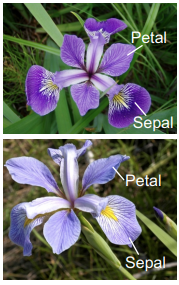
\includegraphics[width=\marginparwidth]{fig1304}\captionof{figure}{Petals and a sepals for Iris versicolor (top) and Iris virginica (bottom). (Photos from Wikipedia)}\label{fig:55}}

\begin{lstlisting}
from sklearn.datasets import load_iris
from sklearn.model_selection import train_test_split

iris = load_iris()
X = iris['data'] #150 entries, 4 parameters each
Y = iris['target'] #150 entries, values of 0, 1, or 2
names = iris['target_names']
feature_names = iris['feature_names']
X_train, X_validate, Y_train, Y_validate \
		= train_test_split(X, Y, test_size=0.333)

\end{lstlisting}

You may want to print out any or all of the defined variables to see what you are
working with.

\begin{problem}\label{P13.5} Develop a neural net which will learn to separate the irises based on the
four characteristics, with training and validation accuracies both over 95 $\%$.\end{problem}
Hint: This problem is much like Example 3 in that it's a classification problem. Here are some specific things you should do which are quite similar to that example:
\begin{itemize}
\item You\rq ll need to import the appropriate keras libraries.
\item Use the np$\_$utils.to$\_$categorical function to turn the outputs which
are 0, 1, or 2 into three separate outputs which are each 0 or 1. You will need
to do this for Y$\_$validate as well as for Y$\_$train.
\item Use a softmax activation function for the final layer, but with 3 nodes as
opposed to 10 nodes
\item Use the categorical$\_$crossentropy cost function
\item Use the adam optimizer
\item Use metrics=['accuracy'] in your compile command
\item  Evaluate your model with X$\_$validate and Y$\_$validate
\end{itemize}
Unlike Example 3, you should not use any convolution layers; instead, do the problem with a fully connected network like Example 2 . You can choose the number of layers (at least 2, though) and the number of nodes in each layer. Also like Example 2, be sure to specify the size of the input layer in your first model.add command. If your network seems to be overfitting the data, as seen by a very high accuracy with the training data but a low accuracy with the validation data, try simplifying your network.
A note on the model compile command: You may have noticed that the mo del. compil e command was used in two slightly different ways for Examples 2 and 3. In Example 2 it was done like this:\\
optimizer$\_$choice = optimizers.adam(lr=0.05)\\
model.compile(loss='mean$\_$squared$\_$logarithmic$\_$error',\\
optimizer=optimizer$\_$choice, metrics=['mse'])\\

Whereas in Example 3 it was like this:\\
model.compile(loss='categorical$\_$crossentropy',\\
optimizer='adam',metrics=['accuracy'])\\

The difference between the two is that if you want to specify any hyperparameters for the optimizer (e.g. adam), such as the learning rate, then you must precede the compile command with an optimizers command as in Example 2 . And then inside the mo del. compil e command you set the optimizer equal to the name of the optimizer variable you have just created, without quotation marks. If, however, you are content to use the default hyperparameters for the optimizer, then inside the model . compile command, you can set the optimizer equal to a string indicating your choice, in quotes.
